\chapter{Introduction}

The Stern-Gerlach (SG) experiment is central to the development and understanding of quantum mechanics. Since it first confirmed the quantization of angular momentum for atomic-scale systems in 1922 \cite{stern}, the SG experiment has occupied debate about the foundations of quantum theory \cite{bocking}.

The SG experiment also provides a versatile base for the discussion of quantum mechanics in general. The purpose of the experiment is to measure the spin angular momentum of electrons. Unlike more complicated quantum systems, the observable values of an electron's spin are discrete and finite. Because the SG experiment exemplifies quantum behavior within a simple context, it is an effective framework for introducing quantum mechanics in an educational setting. This ``spins-first'' approach to teaching quantum mechanics currently shapes curricula \cite{gire} and textbooks \cite{mcintyre}, and is supported by research that reports improved conceptual understanding among students taught with this approach \cite{Sadaghiani}.

The relative simplicity of the SG experiment also provides an initial testing ground for modifications to quantum theory. For a proposed approach to quantum mechanics to be viable, it must (at minimum) reproduce the predictions of the standard approach that agree with experiment. In this thesis, we reproduce these predictions using the \textit{consistent histories} approach to quantum mechanics. In doing so, we continue the conversation about how to interpret the SG experiment, and take advantage of the simplified context to explain \textit{entanglement} in an accessible way.

Existing ``spins-first'' curricula treat the electron's position classically; in doing so, they ignore the entanglement of spin and position degrees of freedom, which characterizes the measurement process for the SG experiment \cite{rodriguez}. This is an intentional simplification, as the purpose of the ``spins-first'' approach is to postpone discussion of position. After the student learns about position, it may be worthwhile to redirect them to the SG experiment to provide a more modern description of quantum measurement, as well as an introduction to entanglement.

This thesis exists as a supplement to a spins-first education for those interested in quantum foundations research. To begin, we revisit the fundamental assumptions of quantum theory and motivate the modification (or elimination) of measurement-related postulates. Then, we propose a unitary measurement model for the SG experiment that relies on less fundamental assumptions than the standard model. We conclude by interpreting the results of SG measurement using the consistent histories approach, which replaces the discarded assumptions in giving the measurement model predictive power.

While the consistent histories approach does not answer the question of \textit{how} or \textit{why} a particular measurement outcome occurs, it reproduces the standard prediction of \textit{how often} it occurs. By doing so without relying on foundational assumptions about measurement, consistent histories can accommodate a more detailed picture of the systems and interactions at play in the measurement process.


\chapter{Stern-Gerlach Experiments}
Numerous explanations of the Stern-Gerlach experiment exist with varying levels of detail and accessibility \cite{mcintyre, bocking, rodriguez, stern}, so we provide only a brief review of the experimental setup and compare schematic diagrams from these accounts in  \autoref{Figure:stern} and \autoref{Figure:new stern}.

The purpose of the experiment is to measure the spin angular momentum of electrons. By spinning along its own axes (like a basketball on a finger), an electron possesses a magnetic moment that interacts with external magnetic fields\footnote{As a point particle, an electron cannot actually spin about its own axes, so ``spin'' is a misnomer. However, electrons do posses an intrinsic magnetic moment, and thinking of its source as internal rotation is useful for building intuition.}. In a Stern-Gerlach apparatus, magnets are configured to create an inhomogeneous magnetic field with a gradient in primarily one direction (conventionally $\hat{z}$). When electrons are sent through this field in a direction perpendicular to the magnetic gradient (conventionally $\hat{y}$), their trajectories are deflected based on the magnitude of their spin in the $\hat{z}$ direction only. After it traverses the magnetic field, the electron's $\hat{z}$ position is measured through collision with a screen. From this, we can deduce the electron's $\hat{z}$ component of spin.

\begin{figure}[!tb]
\centering\CaptionFontSize
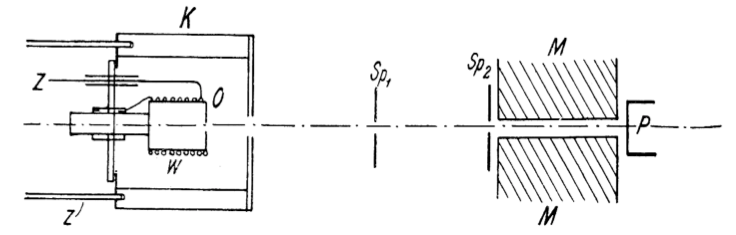
\includegraphics[height=2.0in]
{Figure-stern}
\caption[Otto Stern's scheme for the original Stern-Gerlach experiment]
  {The scheme for the original Stern-Gerlach experiment, from Otto Stern's private collection held at the J.C. Senckenberg Library in Frankfurt, Germany \cite{bocking}. Present are the oven generating the beam of electrons (elements $K,O,W,Z$), collimators (elements $S_p$), magnets (elements $M$), and the detection screen (element $P$).}
\label{Figure:stern}
\end{figure}

\begin{figure}[!tb]
\centering\CaptionFontSize
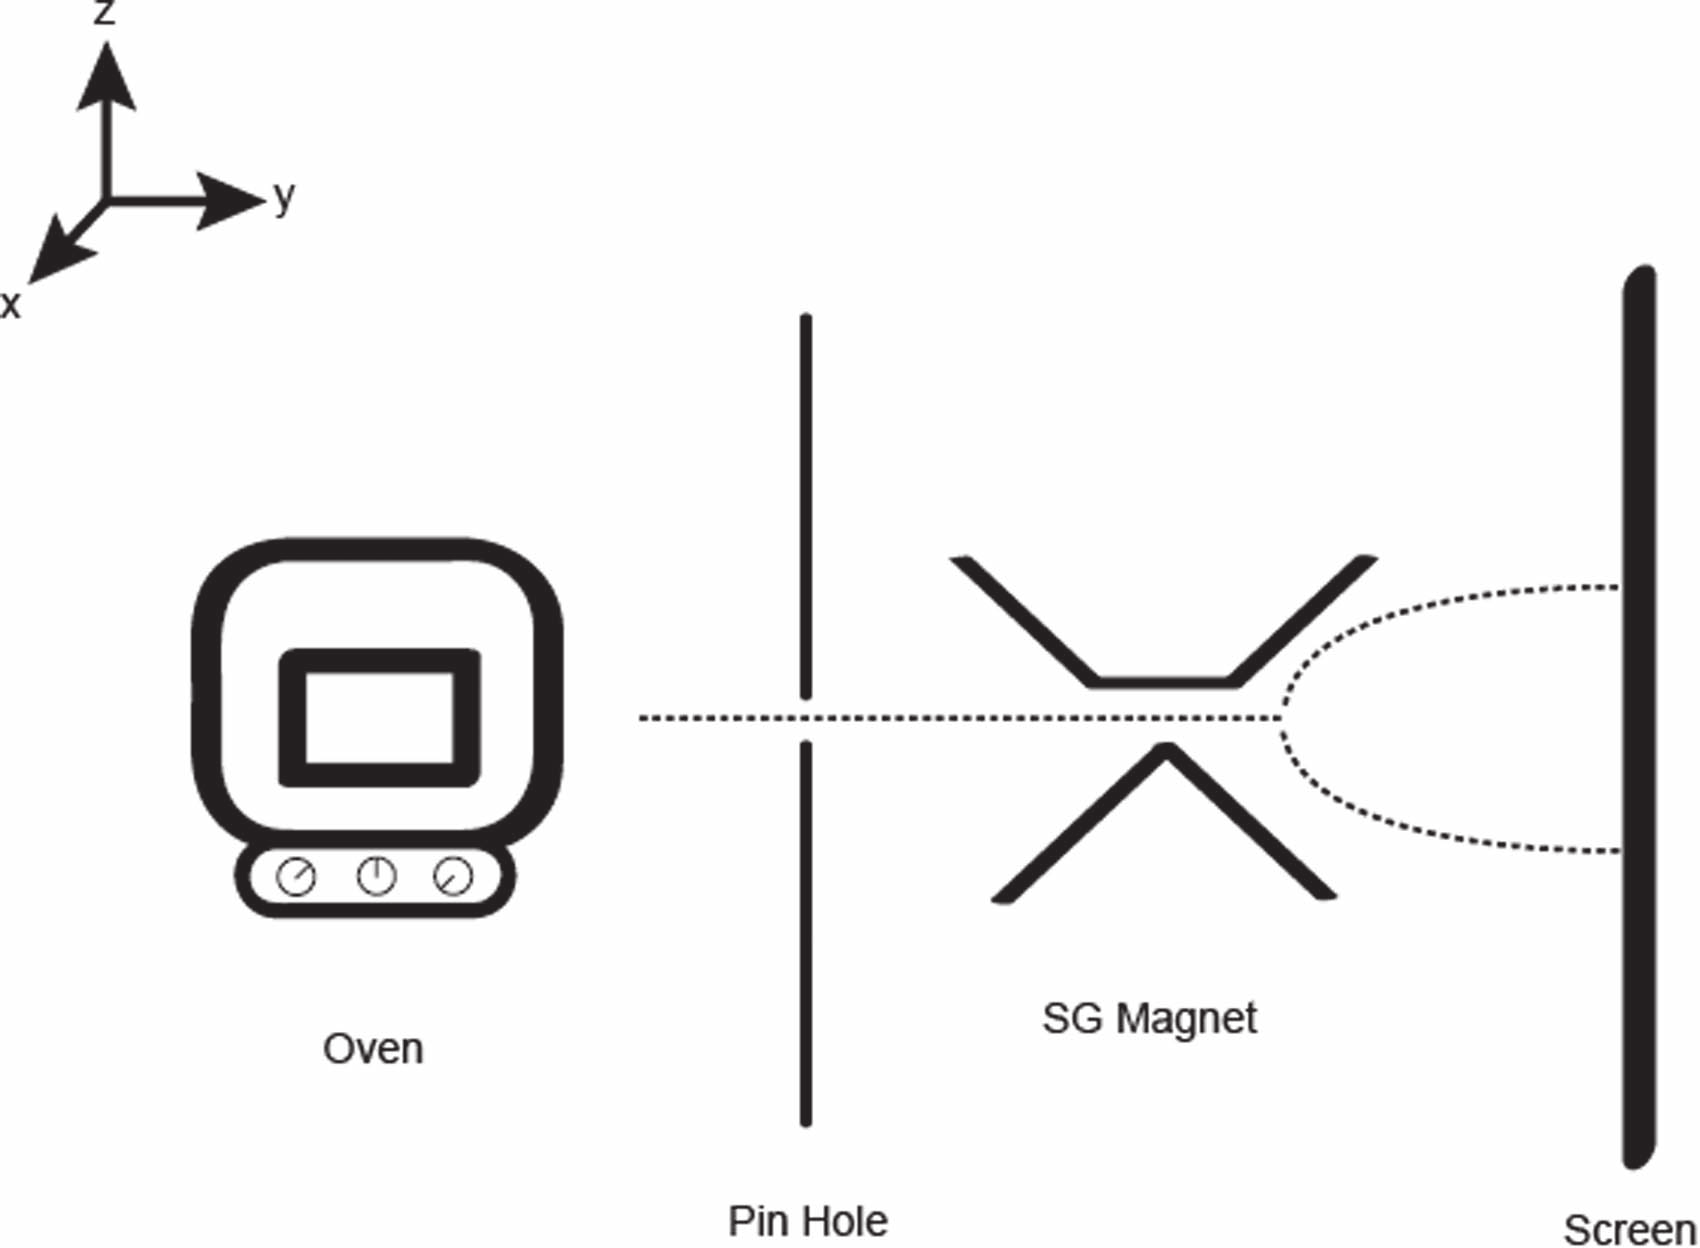
\includegraphics[height=3.0in]
{Figure-new-stern}
\caption[Scheme for the Stern-Gerlach experiment from a modern analysis]
  {The scheme for the Stern-Gerlach experiment adapted from a modern analysis \cite{rodriguez}. Again, the oven, collimator, magnet, and detection screen are pictured. The similarity between this schematic and \autoref{Figure:stern} highlights how the same experimental setup has occupied the discussion of quantum foundations for nearly 100 years.}
\label{Figure:new stern}
\end{figure}

\begin{figure}
\centering\CaptionFontSize
\begin{tikzpicture}[shorten >=1pt,auto, thick,
     square node/.style={rectangle, minimum height=2cm, minimum width=1.50cm, text width = 1.25cm, draw, font=\sffamily\Large\bfseries},
     port/.style={rectangle, draw,  minimum height=1cm, minimum width=0.75cm, font=\sffamily\Large\bfseries},
     wf/.style={rectangle, minimum height=1cm}]
    \apparatus{1}{2}{0}{$\hat{z}$};

    \node(w0) at (-1,0) {$100 \% $ of electrons};
    \node[wf] (w1) at (5, 0.5) {$50 \%$ of electrons};
    \node[wf] (w2) at (5, -0.5) {$50 \%$ of electrons};

    % \node(label1) at (0, -1.75) {$\bm{t_0}$};
    % \node(label2) at (6.25, -1.75) {$\bm{t_1}$};

    \draw[line width=0.5mm] (w0) -- (1);
    \draw[line width=0.5mm] (1+) -- (w1);
    \draw[line width=0.5mm] (1-) -- (w2);
\end{tikzpicture}

\caption[Results of Stern-Gerlach Experiment 1]
{Visualization of the results of SG Experiment 1. The $\hat{z}$ spin values are discrete (shown by the analyzer having only spin-up and spin-down outputs), and an even split of spin-up and spin-down measurements are observed. This result depends on the randomized initial orientation of spin provided by the oven.}
\label{Figure:Exp 1}
\end{figure}

We now introduce three specific SG experimental setups that will be referenced throughout this thesis. These experiments are adapted from those in McIntyre's introductory quantum mechanics text \cite{mcintyre}.
\section{Experiment 1} \label{og experiment 1}
The first experiment measures the $\hat{z}$ component of spin. Because the oven provides a large quantity of electrons with randomly oriented spin, classical mechanics predicts a continuous spread of deflections and corresponding screen collisions. However, in a departure from classical behavior, electrons only collide in two distinct regions of the screen. This is evidence that the spin angular momentum of the electron is \textit{quantized}, meaning that its possible values are restricted. We call these two values \textit{spin-up} and \textit{spin-down}, and observe an even split between spin-up and spin-down measurements. This result is represented schematically in \autoref{Figure:Exp 1}.

In probability theory, a \textit{sample space} consists of an exhaustive set of mutually exclusive outcomes, called \textit{events}. The sample space for Experiment 1 consists of spin-up and spin-down events, both having 50\% probability.

\section{Experiment 2}

For the second experiment, two consecutive SG measurements are made. Electrons are first sent through an apparatus measuring the $\hat{z}$ component of spin, which is configured so that spin-down electrons collide with the screen. The spin-up electrons do not collide with the screen, and are instead routed to another SG apparatus measuring the $\hat{x}$ component of spin. At each apparatus, we find an even split between electrons measured spin-up and spin-down. This result is represented schematically in \autoref{Figure:Exp 2}.

\begin{figure}
\centering\CaptionFontSize
\begin{tikzpicture}[shorten >=1pt,auto, thick,
     square node/.style={rectangle, minimum height=2cm, minimum width=1.50cm, text width = 1.25cm, draw, font=\sffamily\Large\bfseries},
     port/.style={rectangle, draw,  minimum height=1cm, minimum width=0.75cm, font=\sffamily\Large\bfseries},
     wf/.style={rectangle, minimum height=1cm}]
    \apparatus{1}{3}{0}{$\hat{z}$};
    \apparatus{2}{6}{1.5}{$\hat{x}$};

    \node[wf] (w0) at (-0.5,0) {$100 \% $ of electrons};
    \node[wf] (w1) at (9, 2.0) {$25 \%$ of electrons};
    \node[wf] (w2) at (9, 1.0) {$25 \%$ of electrons};
    \node[wf] (w3) at (6, -0.5) {$50 \%$ of electrons};

    \draw[line width=0.5mm] (w0) -- (1);

    \draw[line width=0.5mm] (1+) -- (2);
    \draw[line width=0.5mm] (1-) -- (w3);
    \draw[line width=0.5mm] (2+) -- (w1);
    \draw[line width=0.5mm] (2-) -- (w2);
\end{tikzpicture}

\caption[Results of Stern-Gerlach Experiment 2]
{Visualization of the results of SG Experiment 2. Electrons measured with an up $\hat{z}$ component of spin are routed to a second apparatus, this time oriented to measure the $\hat{x}$ component of spin. Once again, an even split of spin-up and spin-down measurements are observed at the second apparatus.}
\label{Figure:Exp 2}
\end{figure}

If we decide that electrons measured spin-down in the $\hat{z}$ apparatus are uninteresting, we can choose not to count them (reducing our sample size). Re-normalized probabilities are shown in \autoref{Figure:Exp 2 renormalized}.

\begin{figure}
\centering\CaptionFontSize
\begin{tikzpicture}[shorten >=1pt,auto, thick,
     square node/.style={rectangle, minimum height=2cm, minimum width=1.50cm, text width = 1.25cm, draw, font=\sffamily\Large\bfseries},
     port/.style={rectangle, draw,  minimum height=1cm, minimum width=0.75cm, font=\sffamily\Large\bfseries},
     wf/.style={rectangle, minimum height=1cm}]
    \apparatus{1}{3}{0}{$\hat{z}$};
    \apparatus{2}{6}{1.5}{$\hat{x}$};

    \node[wf] (w0) at (-0.5,0) {$100 \% $ of electrons};
    \node[wf] (w1) at (9, 2.0) {$50 \%$ of electrons};
    \node[wf] (w2) at (9, 1.0) {$50 \%$ of electrons};


    \draw[line width=0.5mm] (w0) -- (1);

    \draw[line width=0.5mm] (1+) -- (2);

    \draw[line width=0.5mm] (2+) -- (w1);
    \draw[line width=0.5mm] (2-) -- (w2);
\end{tikzpicture}

\caption[Re-normalized results of Stern-Gerlach Experiment 2]
{Visualization of the results of SG Experiment 2, where $\hat{z}$ spin-down electrons are not counted. These measurements are still made, but we chose to ignore them, reducing our sample size. This setup effectively prepares an electron with $\hat{z}$ spin-up to be measured in the $\hat{x}$ apparatus.}
\label{Figure:Exp 2 renormalized}
\end{figure}

\section{Experiment 3}
The third experiment builds on Experiment 2 by directing the electrons measured spin-up in the $\hat{x}$ apparatus to a third apparatus, which measures the $\hat{z}$ component of spin. The $\hat{z}$ component of spin has already been measured, and electrons measured spin-down were discarded, so we expect all electrons to be measured spin-up in the third apparatus. Instead, we once again find an even split between electrons measured spin-up and spin-down at the second $\hat{z}$ apparatus. This result is represented schematically in \autoref{Figure:Exp 3}.

Classically, the electron's $\hat{z}$ spin would be unaffected by the $\hat{x}$ spin measurement. If the electron retained its measured $\hat{z}$ spin regardless of the measurement of $\hat{x}$ spin, the total sample space would consist of compound events of $\hat{z}$ and $\hat{x}$ spin. That is, we could say that the electron is spin-up/spin-down in the $\hat{z}$ direction \textit{and} spin-up/spin-down in the $\hat{x}$ direction; spin in $\hat{z}$ and $\hat{x}$ directions would have \textit{compatible} sample spaces if their events could be compounded in this way.

However, it appears that the act of measuring the $\hat{x}$ component of spin disturbs the system in such a way that the prior measurement of the $\hat{z}$ component of spin no longer holds. Due to the inability to simultaneously determine these values, spin in $\hat{z}$ and $\hat{x}$ directions have \textit{incompatible} sample spaces; the electron cannot have definite spin values in both $\hat{z}$ and $\hat{x}$ directions at one instant in time. Similar experiments show that spin components in any two non-collinear directions have incompatible sample spaces. Consequently, spin can only be determined along one direction at a time.

\begin{figure}
\centering\CaptionFontSize
\begin{tikzpicture}[shorten >=1pt,auto, thick,
     square node/.style={rectangle, minimum height=2cm, minimum width=1.50cm, text width = 1.25cm, draw, font=\sffamily\Large\bfseries},
     port/.style={rectangle, draw,  minimum height=1cm, minimum width=0.75cm, font=\sffamily\Large\bfseries},
     wf/.style={rectangle, minimum height=1cm}]
     \apparatus{1}{3}{0}{$\hat{z}$};
     \apparatus{2}{6}{1.5}{$\hat{x}$};
     \apparatus{3}{9}{3}{$\hat{z}$};

     \node[wf] (w0) at (-0.5,0) {$100 \% $ of electrons};
     \node[wf] (w2) at (9, 1.0) {$25 \%$ of electrons};
     \node[wf] (w3) at (6, -0.5) {$50 \%$ of electrons};
     \node[wf] (w4) at (12, 3.5) {$12.5 \%$ of electrons};
     \node[wf] (w5) at (12, 2.5) {$12.5 \%$ of electrons};

     \draw[line width=0.5mm] (w0) -- (1);

     \draw[line width=0.5mm] (1+) -- (2);
     \draw[line width=0.5mm] (1-) -- (w3);
     \draw[line width=0.5mm] (2+) -- (3);
     \draw[line width=0.5mm] (2-) -- (w2);
     \draw[line width=0.5mm] (3+) -- (w4);
     \draw[line width=0.5mm] (3-) -- (w5);
\end{tikzpicture}

\caption[Results of Stern-Gerlach Experiment 3]
{Visualization of the results of SG Experiment 3. Notice that even though $\hat{z}$ spin-up had already been measured for all electrons routed the the third apparatus, it still measures an even split of spin-up and spin-down electrons. The electron ``forgetting'' its previous measurement of $z$ spin reflects the fundamental inability to simultaneously determine $S_z$ and $S_x$.}
\label{Figure:Exp 3}
\end{figure}
